\chapter{Implementierte Funktionen}
Wie im Vorherigen Kapitel bereits angesprochen wurde, nutzt Rivescript Routinen, die aus den .rive-Dateien angesprochen werden können. Diese Routinen müssen dem Chatbot bekannt gemacht werden. Im Folgenden sollen die Funktionen, die der Chatbot unterstützt, vorgestellt werden und auf deren Implementierung eingegangen werden.

\section{Hochschulbezogene Funktionen}
Der Chatbot hat die Hauptaufgabe mit natürlichen Texteingaben Informationen über die Hochschule bereitzustellen. Diese Informationen enthält der Chatbot über Abfragen der hochschuleigenen REST-API. Der Chatbot deckt die Themengebiete Mensa, Stundenplan, Informationen über Lehrende und Vorlesungen ab.

\subsection{Mensa}
Die Mensafunktion war bislang bereits vom Bot abgedeckt, indem man /mensa aufruft. Dabei erscheint ein Menü, welches dem Benutzer eine Auswahlmöglichkeit gibt, innerhalb der nächsten fünf Tage inklusive des heutiges Tages, falls es ein ''Arbeitstag'', also ein Tag außer Samstag und Sonntag ist, das Mensaangebot zu einem bestimmten Tag ausgeben zu lassen.
Der Chatbot ermöglicht nun zunächst diese Funktionalität im normalen Sprachgebrauch zu benutzen. Dabei werden Formulierungen nach konkreten Tagen ''Was gibt es am Montag in der Mensa?'' und vom heutigen Tag ausgehend ''Was gibt es heute/morgen/übermorgen in der Mensa?''. Es gibt auch die Möglichkeit nach vergangenen Tagen zu fragen, dann dementsprechend mit der Vergangenheitsform. Insgesamt wurde definiert, dass wenn der User keinen konkreten Tag angibt, immer der heutige Tag zurückgegeben wird. Das klassische Beispiel wäre ''Was gibt es zu essen?'', bei dem dann das heutige Mensaangebot zurückgegeben wird.
Dies deckt die Basisfunktionalität von dem bestehenden Telegram-Command /mensa ab.

Viel interessanter ist es jedoch für den Benutzer, innerhalb der Gerichte des Mensaangebots filtern zu können. So können die Benutzer zum Beispiel fragen, welche Gerichte vegetarisch und vegan sind. Weitere Fragen im Bezug auf enthaltene Lebensmittel in den Mensaspeisen sind möglich.
In diesem Zusammenhang haben sich Schwierigkeiten mit der Verwendung von Rivescript ergeben. \\
Es werden im Bezug auf die Mensaanfragen des Benutzers zwei Parameter erwartet:
\begin{enumerate}[noitemsep]
    \item der Tag, zum Beispiel ein konkreter Wochentag oder gestern / heute / morgen
    \item eine Lebensmitteleinschränkung, zum Beispiel vegan, ohne Fleisch oder mit Rind 
\end{enumerate}
Diese beiden Parameter können in beliebiger Reihenfolge auftreten, da sowohl die Kombination 
''Was gibt es morgen Vegetarisches in der Mensa?'' und
''Welche vegetarischen Gerichte gibt es morgen zu essen''?
auftreten können. \\
Ein Problem ergibt sich dadurch, dass die Reihenfolge dieser beiden Informationen nicht festgelegt ist. So ist nötig, alle übergebenen Parameter nach einer Tagesinformation zu durchsuchen. Man muss also erst den Typ des Parameters herausfinden, um ihn an Methoden weiterzugeben. \\
Ein weiteres Problem tritt auf, wenn ein der Parameter aus mehreren Wörtern besteht, zum Beispiel “ohne Fleisch”. Rivescript trennt Parameter, die es unter dem *-Wildcard erkennt am Leerzeichen auf. Es ist also nötig, diese wieder nach dem Matchen und vor der Auswertung zusammen zu setzen. \\
Als Strategie wurde eingesetzt, dass man die Parameter nach den Schlüsselwörtern \emph{mit} und \emph{ohne} durchsucht und diese mit den darauf folgenden Wörtern wieder zu einem gemeinsamen String zusammenfügt, bevor man diesen weiter verarbeitet. Dabei ist zu beachten, dass alle Informationen über den gewünschten Tag der Mensaausgabe dort herausgefiltert werden, damit sie nicht im konkatenierten Lebensmittel-String landen. Es sind also viele String-Vergleiche und Konkatenationen notwendig, um die Benutzereingaben sinnvoll auszuwerten. \\
Wenn kein bestimmter Tag gewünscht wird, wird der heutige Tag ausgegeben. Wenn kein bestimmter Lebensmittelwunsch besteht, werden alle Gerichte ausgegeben.

\subsection{Stundenplan}
Der Stundenplan ist eine Funktionalität, die bis jetzt nicht vom IWINewsBot unterstützt wurde. Die Funktionalität wird ebenfalls über die REST-API der Hochschule bezogen. Für die Abfrage müssen Studiengang, Semester und eine eventuelle Gruppe oder Vertiefungsrichtung angegeben werden. Zu diesem Zweck wurden die Einstellungen komplett überarbeitet und an einem Ort, dem Command /settings, zusammengeführt. Ergänzt wurde die Möglichkeit, den aktuellen Studiengang, sein Semester und eine Vertiefungsrichtung im Master anzugeben, die für die Stundenplanabfrage genutzt wird.
Der Stundenplan kann über den Chatbot entweder komplett oder tageweise abgefragt werden.

\subsection{Lehrende}
Zu den Lehrenden wurden zwei verschiedene Abfragemöglichkeiten implementiert. Beide Varianten beziehen ihre Informationen aus der REST-API der Hochschule und benötigen keine Übergabeparameter. 
Die erste Abfragemöglichkeit dient dazu, Informationen über den angefragten Professor, im Speziellen zu den Sprechzeiten, bereitzustellen. Zusätzlich werden dann noch die E-Mail-Adresse, falls vorhanden auch ein kleiner Kommentar des Professors und die Raumnummer des Büros mitausgegeben. Diese Routine bildet also die schon vorher vorhandene Funktion ab, die mit /profs aufgerufen wurde. Um so eine Anfrage abzuschicken, eignet sich zum Beispiel ''Wie lautet die E-Mail von Frau Laubenheimer?'' oder ''Wann hat Professor Vogelsang Sprechstunde?'' \\
Um genügend Spielraum zu geben, wurde für die Anrede ein Platzhalter gewählt, der verschiedene Möglichkeiten abdeckt. Die Ausgabe hierzu kann wie folgt aussehen:

\begin{figure}[!htb]
    \centering
    \caption{Informationen über Lehrende}
      
\includegraphics[width=0.5\linewidth]{Prof.png}
      \label{img:profuebersicht}
    \caption*{Quelle: Eigene Abbildung}
\end{figure}

Die zweite Abfragemöglichkeit wurde komplett neu implementiert und gibt für die angefragten Lehrenden alle Vorlesungen aus, die diese halten. Hierbei wird auf eine erweiterte Abfrage der gleichen REST-Schnittstelle wie bei der Sprechzeitenabfrage zugegriffen. Eine Anfrage im Chatbot kann zum Beispiel sein: ''Welche Vorlesungen hält Professor Henning?'' worauf dann folgende Ausgabe gemacht wird (Vorlesungen mit gleichem Namen, die aber in zwei verschiedenen Studiengängen/Semestern gehalten werden, werden nicht doppelt aufgeführt):

\begin{figure}[!htb]
    \centering
    \caption{Alle Veranstaltungen eines Lehrenden}
      
\includegraphics[width=0.5\linewidth]{Vorlesungsuebersicht.png}
      \label{img:vorlesungsuebersicht}
    \caption*{Quelle: Eigene Abbildung}
\end{figure}

\subsection{Vorlesungen}
Für die Vorlesungen wurde eine neue Routine entwickelt, die für die angefragte Vorlesung den Raum und die Zeit ausgibt. Hierfür müssen über die REST-API der Hochschule gleich zwei verschiedene Objekte abgefragt werden. Zum einen werden alle Stundenpläne abgeholt und zum anderen werden alle Blockkurse abgeholt, da diese nicht in den eigentlichen Stundenplänen mit enthalten sind. Als Ausgabe bekommt man dann die Zeit und den Raum der Vorlesung, wobei die Ausgaben leicht unterschiedlich aussehen, da zwischen ''normaler'' Vorlesung und Blockkurs unterschieden werden muss.

\begin{figure}[!htb]
    \centering
    \caption{Ausgabe von Zeit und Raum von Blockkursen und regulären Veranstaltungen}
    \begin{subfigure}{.5\textwidth}
        \centering
        \caption{Blockkurs}
          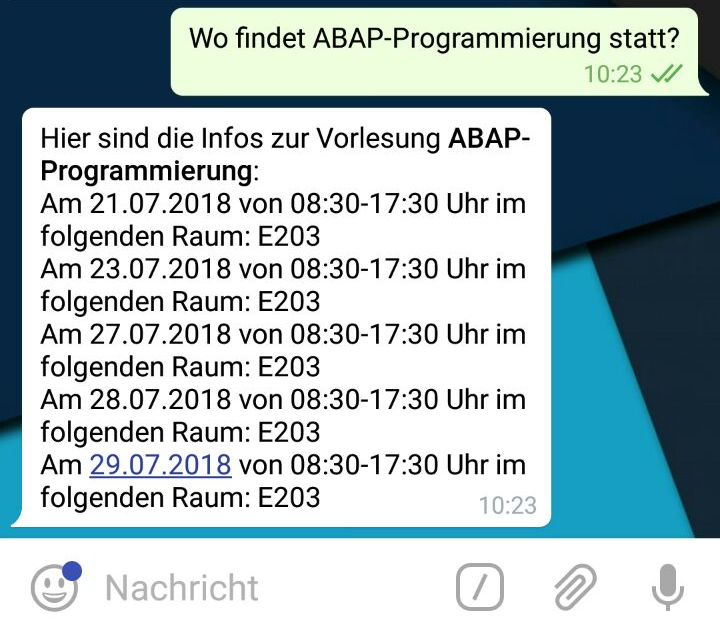
\includegraphics[width=0.9\linewidth]{BlockkursLocation.png}
          \label{img:blockkurs}
    \end{subfigure}%
    \begin{subfigure}{.5\textwidth}
        \centering
        \caption{Reguläre Vorlesung}
          
\includegraphics[width=0.9\linewidth]{VorlesungLocation.png}
          \label{img:vorlesung}
    \end{subfigure}
    \caption*{Quelle: Eigene Abbildung}
    \label{fig:blockkursUndVorlesung}
    \end{figure}

\section{Spaßige Bemerkungen}
Eine weitere Anforderung war es, neben den informativen Anfragen auch auf nicht ernste Anfragen zu antworten. Hierfür wurde eine zusätzliche Datei (fun.rive) angelegt, die neben spitzen Antworten auch einige Informatikerwitze enthält. Neben dem Klassiker ''Was ist der Sinn des Leben?'' antwortet der Bot auf die Anfrage ''Was hast Du an?'' mit ''Das ist ja eine indiskrete Frage''. \\
Durch diesen Ansatz soll erreicht werden, dass Nutzer den Bot gerne benutzen und neue Funktionen entdecken. Die Handhabung soll spielerisch erfolgen und Spaß machen.

\section{Keine gefundene Übereinstimmung}
Für den Fall, dass der Chatbot keine passende Antwort parat hat, ist es möglich generelle Antworten zu geben. Um dies zu ermöglichen wird auf * gematcht. Man kann also standardmäßig mit Floskeln wie ''Ich habe das nicht verstanden'' antworten, damit der User weiß, dass er seine Frage umformulieren muss oder die geforderte Funktion nicht implementiert wurde. Um hierdurch potentielle Features zu finden, sollten diese Anfragen gesondert geloggt werden, damit man alle möglichen Anfragen auch später einfach einsehen kann und neue Funktionen erkennen kann. \\
Der IWINewsBot setzt bereits auf Logback als Logging Framework um Fehler zu finden und aussagekräftige Log-Dateien zu schreiben. Logback hat ein tolles Feature, was es erlaubt auf bestimmte Filter zu reagieren. So kann man bestimmte Log-Nachrichten taggen und diese Tags dann filtern. Das Taggen wird im Code vorgenommen, das Filtern nach Tags geschieht in der logback.xml (Konfigurations-)datei. Hier kann festgelegt werden, dass alle Log-Nachrichten mit einem bestimmten Tag in eine spezielle Datei geschrieben werden.
\lstinputlisting[language=scala, style=scala, numbers=none, caption=Logging der Usereingaben, label=logging, firstline=39, lastline=41]{Chat.scala}

In dem obigen Beispiel werden zwei Nachrichten mit dem Level INFO geloggt. Diese werden mit dem ChatBotMarker getaggt. Bei dem ChatBotMarker handelt es sich um ein Tag, das alle Log-Nachrichten als Chatbot-Nachrichten taggt. Nach diesem Tag kann dann in der Logback-Konfiguration wie folgt gefiltert werden:
\lstinputlisting[language=buildSbt, style=buildSbt, caption=Ausschnitt der logback.xml, label=logback]{logback.xml}

Logback arbeitet mit Appendern, die es ermöglichen, dass Nachrichten auf verschiedenen Ebenen in verschiedene Dateien und Streams geschrieben werden können. Der Chatbot Appender filtert alle Nachrichten nach dem Chatbot-Tag und schreibt diese Nachrichten in die Datei chatbot.log. Alle anderen Log-Nachrichten werden von diesem Appender ignoriert.

Durch diese Logging-Maßnahmen ist es also möglich, alle Anfragen die an den Chatbot gehen zu loggen. Nun sollten aber speziell Anfragen geloggt werden, die der Bot nicht beantworten kann. Hierzu wurde für denn Fall * in der .rive-Datei eine spezielle Routine gestartet, die NoComprendoRoutine:
\lstinputlisting[numbers=none, caption=Eine Routine wird beim Nicht-Verstehen aufgerufen, label=matchingStar, firstline=24, lastline=26]{riveExamples.rive}

Das Verhalten dieser Routine ist sehr einfach. Es werden hier einfach programmatisch verschiedene Antworten festgehalten und die Anfrage wird mit dem Logging-Level ERROR geloggt.
\lstinputlisting[language=scala, style=scala, caption=Ausschnitt aus der Always-Match-Routine, label=noComprendo]{NoComprendoRoutine.scala}